\newpage

\section{Induction Variables and Strength Reduction}
Strength reduction is an optimization technique which substitutes expensive operations with computationally cheaper ones. For example, a very weak strength reduction algorithm can substitute the instruction 
\texttt{b = a * 4} with \texttt{b = a << 2}.

\subsection{Motivation}

Opportunities for strength reduction arise routinely from details that the compiler
inserts to implement source-level abstractions. To see this, consider the simple
code fragment shown in Figure \ref{fig:p74-76}. Figure \ref{fig:p74} shows source code and the same loop in a low-level intermediate code.
 Notice the instruction sequence that begins at the label L2. The compiler inserted this code
(with its multiply) as the expansion of A[i]. Figure \ref{fig:p75}  shows the code that results from applying Strength Reduction,
Figure \ref{fig:p76} is followed by dead-code elimination. The compiler created a new variable, t2$^\prime$, to
hold the value of the expression i $*$ 4 + A. Its value is computed directly, by
incrementing it with the constant 4, rather than recomputing it on each iteration
as a function of i. Strength reduction automates this transformation. 

\begin{figure}[H]
    \centering
    \begin{subfigure}{0.6\textwidth}
    \centering
        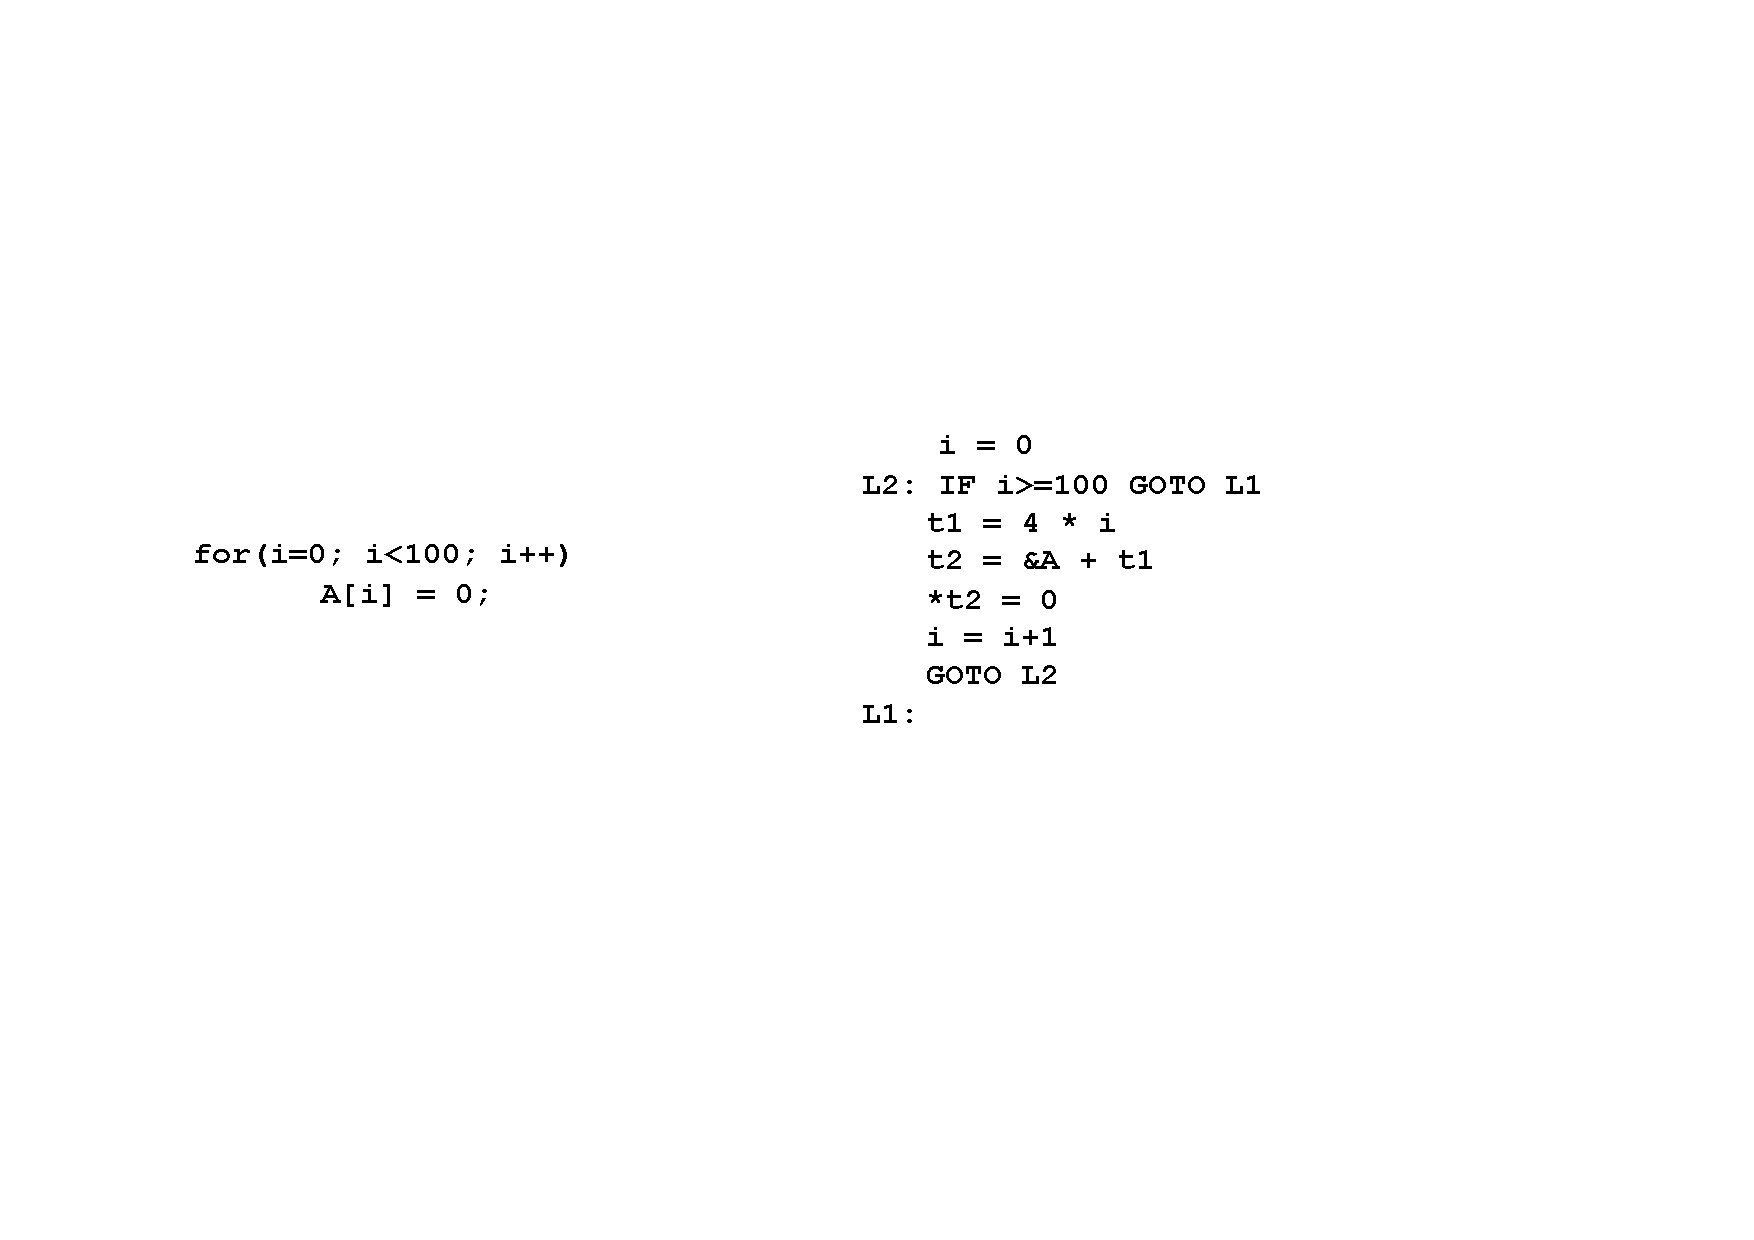
\includegraphics[width=\textwidth]{p74.pdf}
        \caption{Origianl code.}
        \label{fig:p74}
    \end{subfigure}
    \begin{subfigure}{0.6\textwidth}
    \centering
        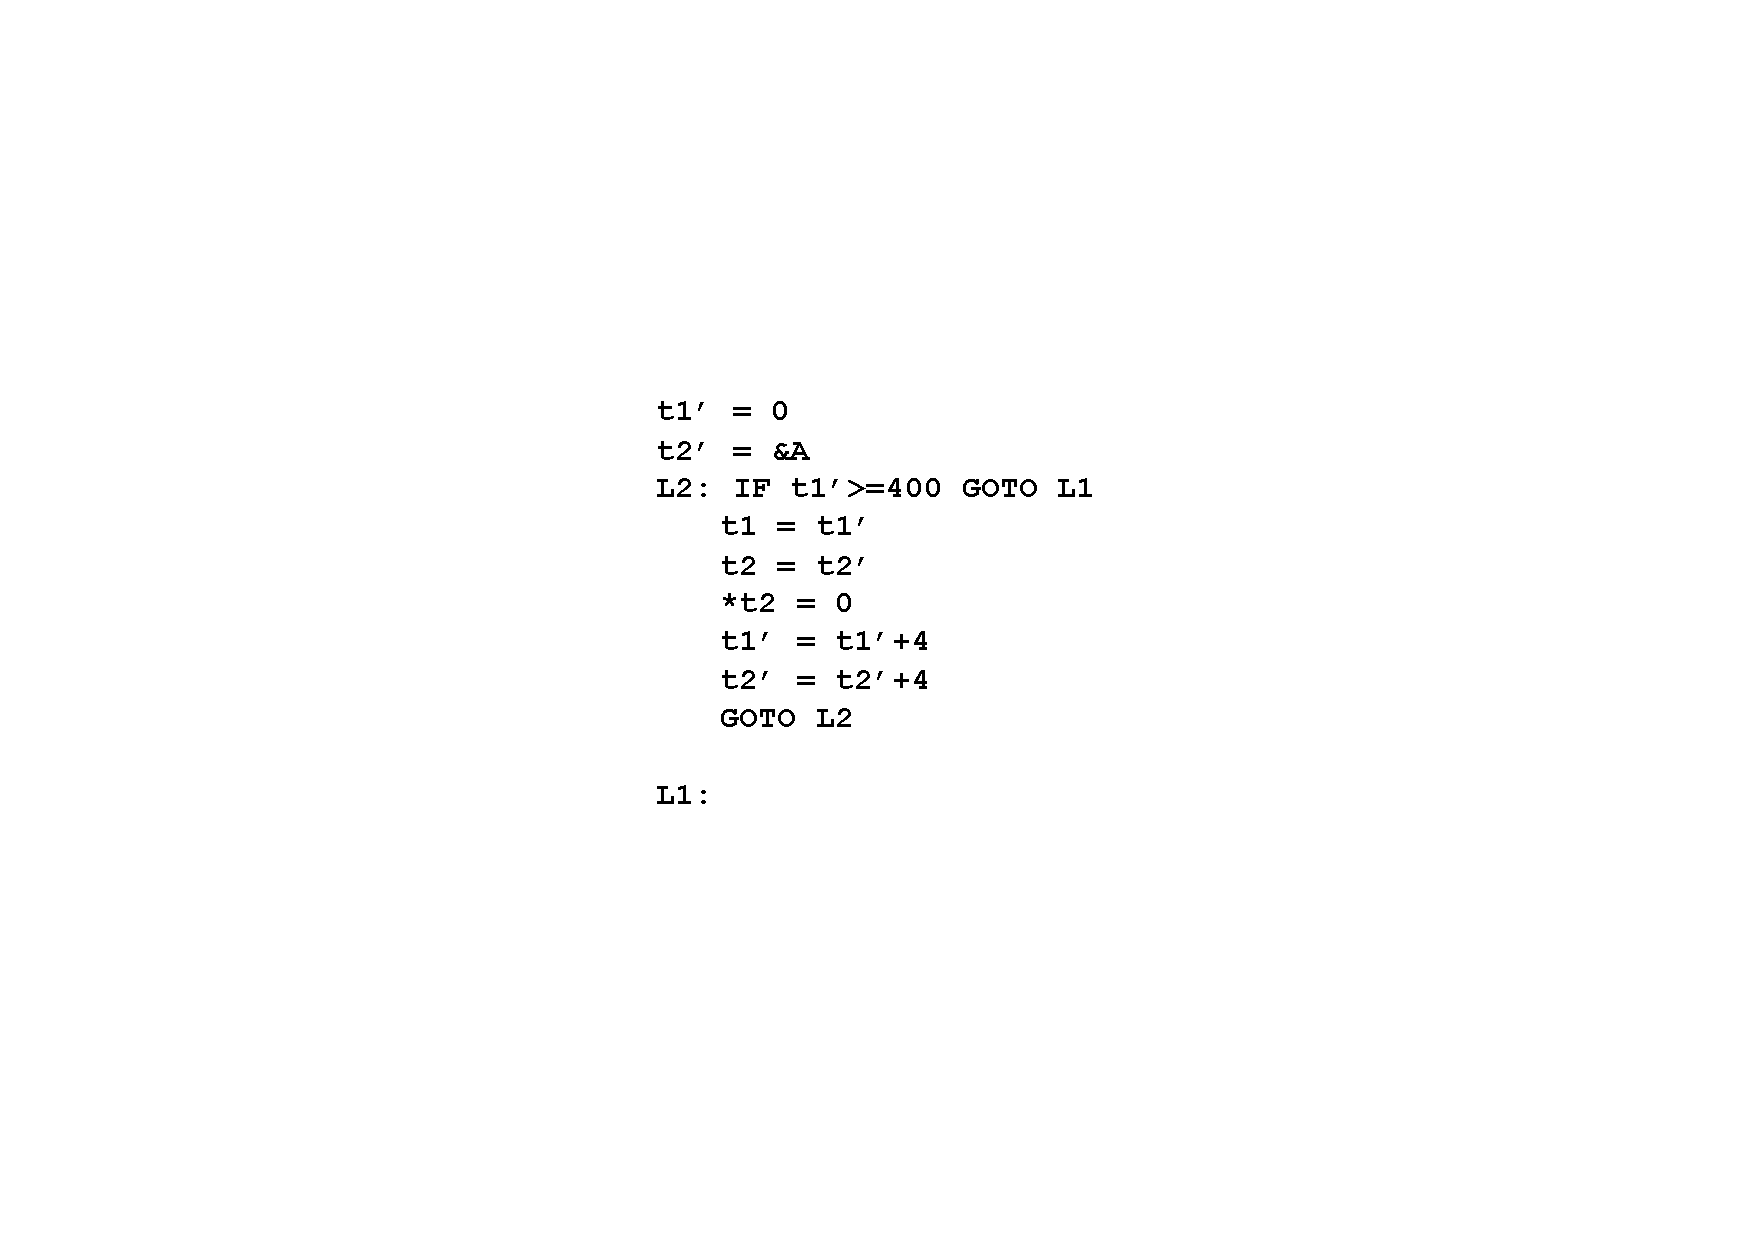
\includegraphics[width=\textwidth]{p75.pdf}
        \caption{After induction variable substitute.}
        \label{fig:p75}
    \end{subfigure}
    \begin{subfigure}{0.6\textwidth}
        \centering
            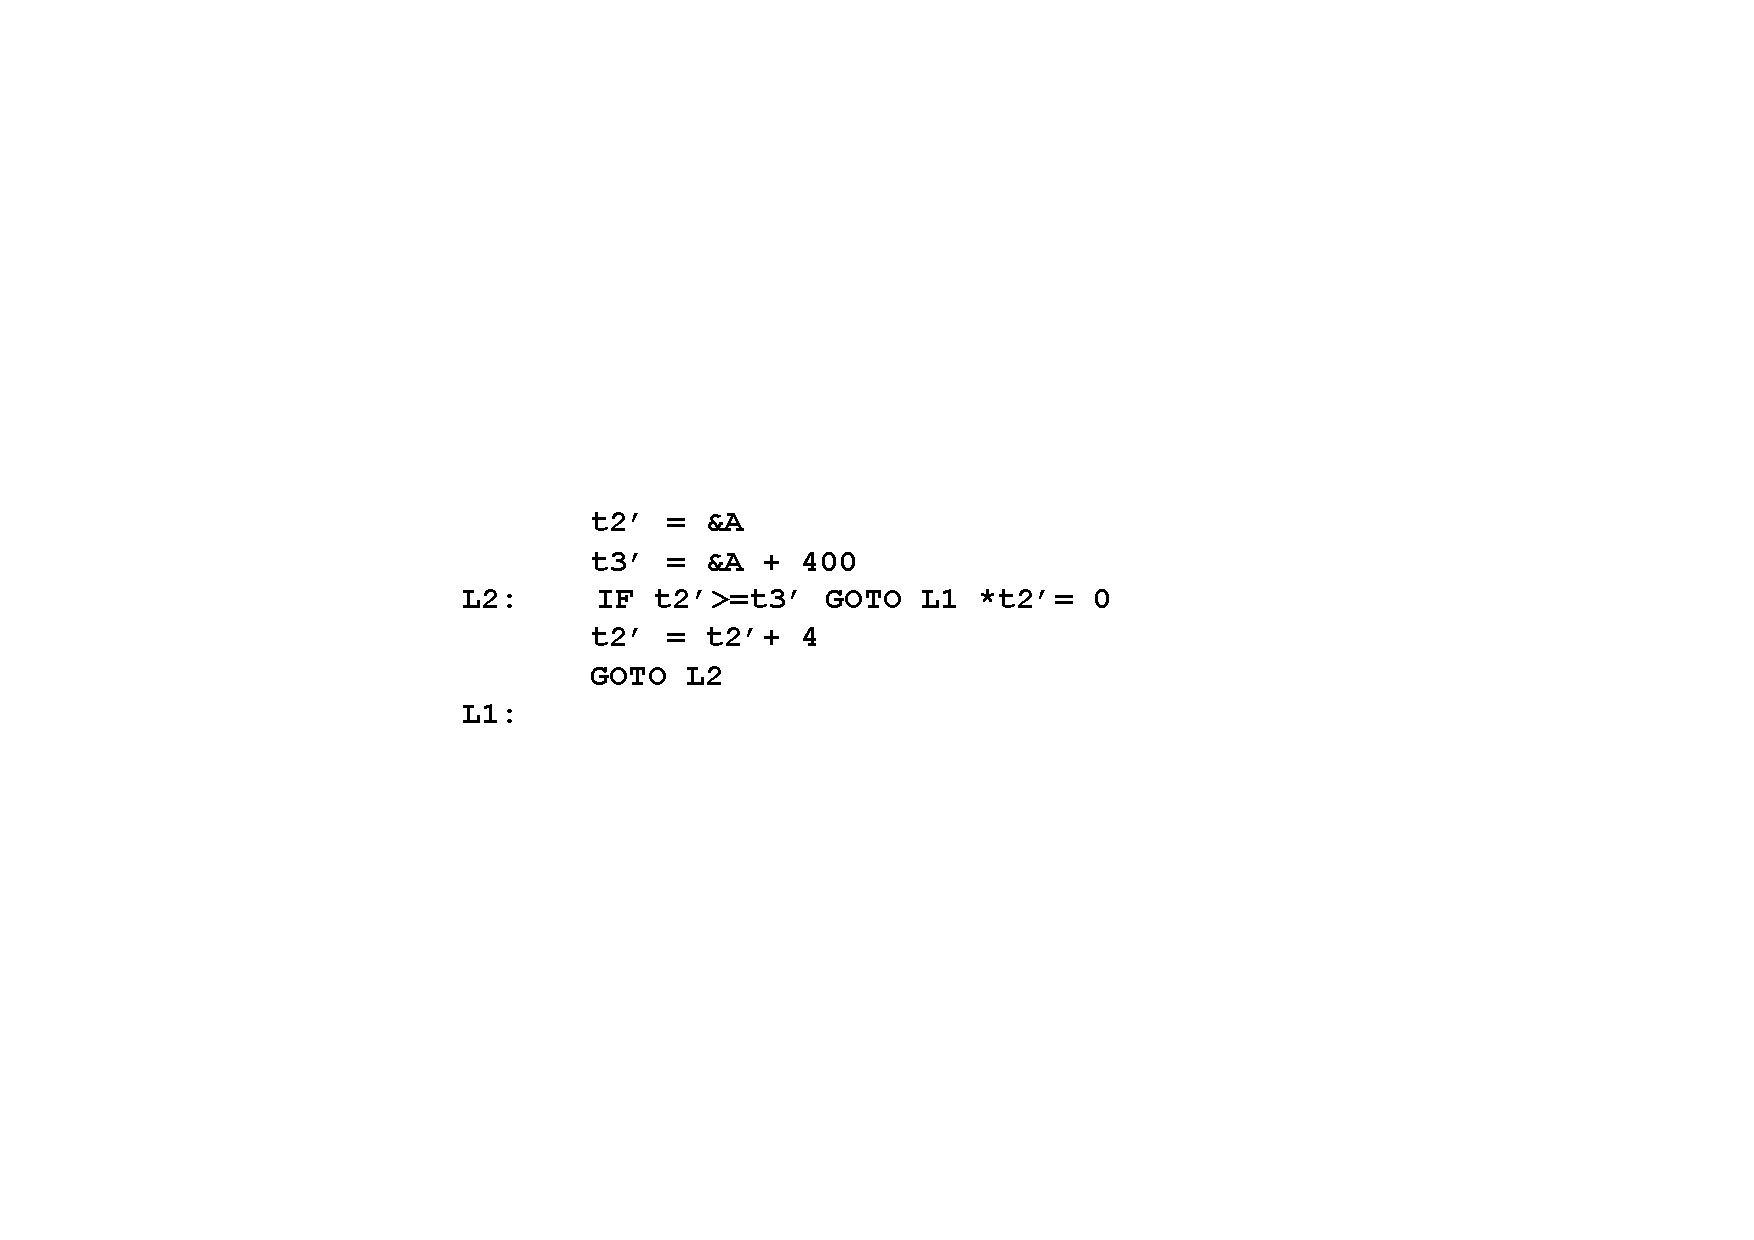
\includegraphics[width=\textwidth]{p76.pdf}
            \caption{Final code.}
            \label{fig:p76}
        \end{subfigure}
    \caption{An example of strength reduction.}
       \label{fig:p74-76}
\end{figure}



\subsection{Definitions}

\begin{definition}{Basic Induction Variable}
    A basic induction variable (e.g., i as shown in Figure \ref{fig:p74} ) is a variable X whose only definitions within the loop
are assignments of the form: X = X+c or X = X-c, where c is either a constant or 
a loop-invariant variable. 
\end{definition}

\begin{definition}{Induction Variable}
    An induction variable is either a basic induction variable B, or
or a variable defined once within the loop (e.g., t1,t2 as shown in Figure \ref{fig:p74} ) , whose value is a linear function
of some basic induction variable at the time of the definition:
$A = c_1 * B + c_2$
\end{definition}

The FAMILY of a basic induction variable B is the set of induction variables A such that each time A is assigned in the loop,
the value of A is a linear function of B. (e.g., t1, t2 is in family of i as shown in Figure \ref{fig:p74})


\subsection{Optimizations}

\subsubsection{Strength Reduction}
\begin{algorithm}[H]
    \caption{Strength Reduction Optimizations}\label{alg:Strength Reduction Optimizations}
    \begin{algorithmic}


    \State{A is an induction variable in family of basic induction variable B (i.e., $A = c_1 * B + c_2$ )}
    \State{\,\,\,\,\,\,\,\, Create new variable A$^\prime$}
    \State{\,\,\,\,\,\,\,\, Initialize in preheader A$^\prime$ = $c_1 * B + c_2$}
    \State{\,\,\,\,\,\,\,\, Track value of B: add after $B=B+x$: $A^\prime=A^\prime+x*c_1$}
    \State{\,\,\,\,\,\,\,\, Replace assignment to A: replace lone $A=\dots$ with $A=A^\prime$}
    \end{algorithmic}
    \end{algorithm}

\subsubsection{Optimizing non-basic induction variables}


\begin{itemize}
\item copy propagation
\item dead code elimination
\end{itemize}


\subsubsection{Optimizing basic induction variables}